\documentclass[11pt]{article}

\usepackage[margin=0.9in]{geometry}
\usepackage[T1]{fontenc}
\usepackage[utf8]{inputenc}
\usepackage{lmodern}
\usepackage{microtype}
\usepackage{xcolor}
\usepackage{graphicx}
\usepackage{booktabs}
\usepackage{tabularx}
\usepackage{array}
\usepackage{caption}
\usepackage{hyperref}
\usepackage{tikz}
\usepackage{fancyhdr}
\usepackage{eurosym}
\usepackage{longtable}
\usepackage[numbers,sort&compress]{natbib}

\usetikzlibrary{arrows.meta,positioning,fit,backgrounds,calc}

\definecolor{eirink}{HTML}{17313A}
\definecolor{eirblue}{HTML}{2D6678}
\definecolor{eirsand}{HTML}{F4EFE4}
\definecolor{eirgold}{HTML}{E1A33A}
\definecolor{eirmist}{HTML}{DCE7E5}
\definecolor{eirrose}{HTML}{D9785C}
\definecolor{eirslate}{HTML}{5C7883}

\hypersetup{
  colorlinks=true,
  linkcolor=eirblue,
  citecolor=eirblue,
  urlcolor=eirblue,
  pdftitle={A Computational View of Medicine},
  pdfauthor={Birger Moëll and Erica Hughberg}
}

\setlength{\parindent}{0pt}
\setlength{\parskip}{0.55em}
\setlength{\headheight}{14pt}
\renewcommand{\familydefault}{\sfdefault}
\pagestyle{fancy}
\fancyhf{}
\lhead{\textcolor{eirslate}{A Computational View of Medicine}}
\rhead{\textcolor{eirslate}{Moëll \& Hughberg}}
\cfoot{\textcolor{eirslate}{\thepage}}
\renewcommand{\headrulewidth}{0pt}

\captionsetup{
  font=small,
  labelfont={bf,color=eirink},
  textfont={color=eirslate}
}

\newcommand{\summarybox}[1]{%
  \begin{center}
  \fcolorbox{eirgold}{eirsand}{\parbox{0.93\linewidth}{#1}}
  \end{center}
}

\newcommand{\calloutbox}[2]{%
  \begin{center}
  \fcolorbox{eirmist}{white}{\parbox{0.93\linewidth}{\textbf{\textcolor{eirink}{#1}}\par #2}}
  \end{center}
}

\begin{document}

\begin{titlepage}
\pagenumbering{gobble}
\pagecolor{white}
\color{eirink}
\vspace*{1.5cm}

{\fontsize{30}{32}\selectfont\bfseries
A Computational View of Medicine\par}
\vspace{0.45cm}
{\Large Why AI will matter most where disease becomes a search problem\par}
\vspace{0.9cm}
{\large Birger Mo\"ell and Erica Hughberg\\Co-Founders, Eir Space\par}
\vspace{0.35cm}
{\normalsize March 17, 2026\par}

\vfill

\summarybox{
\textbf{Thesis.} The most important medical use of advanced AI is not generic automation. It is high-context reasoning over difficult, patient-specific problems where better synthesis can change diagnosis, treatment choice, escalation, or trial matching. In these settings, disease is better understood as a computational burden distributed across time, modalities, and decision branches than as a static label alone.
}

\vfill

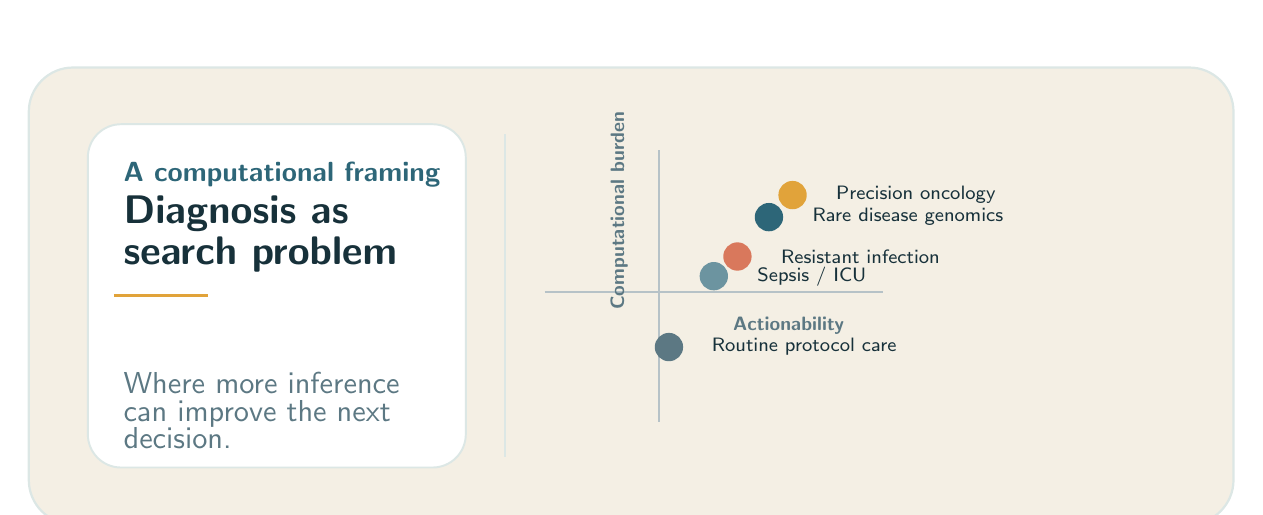
\begin{tikzpicture}[x=1cm,y=1cm]
  \fill[eirsand, rounded corners=16pt] (0,0) rectangle (15.3,5.8);
  \draw[eirmist, line width=0.8pt, rounded corners=16pt] (0,0) rectangle (15.3,5.8);

  \fill[white, rounded corners=12pt] (0.75,0.72) rectangle (5.55,5.08);
  \draw[eirmist, line width=0.7pt, rounded corners=12pt] (0.75,0.72) rectangle (5.55,5.08);
  \node[anchor=north west, font=\bfseries\fontsize{10}{12}\selectfont, text=eirblue] at (1.08,4.72)
    {A computational framing};
  \node[anchor=north west, font=\bfseries\fontsize{15}{18}\selectfont, text=eirink] at (1.08,4.3)
    {Diagnosis as};
  \node[anchor=north west, font=\bfseries\fontsize{15}{18}\selectfont, text=eirink] at (1.08,3.78)
    {search problem};
  \draw[eirgold, line width=1.1pt] (1.08,2.9) -- (2.28,2.9);
  \node[anchor=north west, font=\fontsize{10.5}{13}\selectfont, text=eirslate] at (1.08,2.05)
    {Where more inference};
  \node[anchor=north west, font=\fontsize{10.5}{13}\selectfont, text=eirslate] at (1.08,1.7)
    {can improve the next};
  \node[anchor=north west, font=\fontsize{10.5}{13}\selectfont, text=eirslate] at (1.08,1.35)
    {decision.};
  \draw[eirmist, line width=0.7pt] (6.05,0.86) -- (6.05,4.95);

  \begin{scope}[shift={(8.55,3.0)}]
    \draw[eirslate!45, line width=0.8pt] (-0.55,-1.7) -- (-0.55,1.75);
    \draw[eirslate!45, line width=0.8pt] (-2.0,-0.05) -- (2.3,-0.05);
    \node[font=\scriptsize\bfseries, text=eirslate] at (1.1,-0.48) {Actionability};
    \node[font=\scriptsize\bfseries, text=eirslate, rotate=90] at (-1.05,0.98) {Computational burden};
    \fill[eirgold] (1.15,1.18) circle (0.18);
    \node[anchor=west, font=\scriptsize, text=eirink] at (1.58,1.18) {Precision oncology};
    \fill[eirblue] (0.85,0.9) circle (0.18);
    \node[anchor=west, font=\scriptsize, text=eirink] at (1.28,0.9) {Rare disease genomics};
    \fill[eirrose] (0.45,0.4) circle (0.18);
    \node[anchor=west, font=\scriptsize, text=eirink] at (0.88,0.4) {Resistant infection};
    \fill[eirblue!70] (0.15,0.15) circle (0.18);
    \node[anchor=west, font=\scriptsize, text=eirink] at (0.58,0.15) {Sepsis / ICU};
    \fill[eirslate] (-0.42,-0.75) circle (0.18);
    \node[anchor=west, font=\scriptsize, text=eirink] at (0.0,-0.75) {Routine protocol care};
  \end{scope}
\end{tikzpicture}

\end{titlepage}
\nopagecolor
\clearpage
\pagenumbering{arabic}

\begin{abstract}
Artificial intelligence will not improve every part of medicine equally. Its highest-value role is in disease settings where the bottleneck is not data collection or workflow automation but high-context reasoning over multimodal evidence under uncertainty. We argue for a computational view of medicine that treats serious illness as a search problem over longitudinal records, pathology, imaging, genomics, patient-generated data, treatment history, and branching therapeutic options. The key question is not whether a model can produce clinically fluent text, but whether additional inference changes the next real decision for a specific patient. This constraint applies to clinicians and AI systems alike: both face the same search problem, and the quality of the search depends on the depth and structure of reasoning applied. We synthesize evidence from precision oncology, rare-disease genomics, antimicrobial discovery, sepsis surveillance, pharmacogenomics, psychiatric treatment selection, patient-reported outcomes, open-notes adoption, and N-of-1 medicine. Patient access to records is necessary but insufficient; because clinical reasoning is distributed across specialists and institutions---with the patient as the only persistent entity---data access becomes powerful only when patients and clinicians can repeatedly compute over the full timeline of illness. The result is a framework for directing AI toward cases where reasoning is the bottleneck, outcomes depend on synthesis quality and calibration, and patient-held data can become a force multiplier.
\end{abstract}

\section{Introduction}
Medicine is organized around disease labels, organ systems, and specialty workflows. These abstractions are useful but obscure where the real difficulty lies. In the cases that matter most, the limiting factor is neither the absence of a diagnosis code nor a single decisive test. It is the burden of synthesis: reconciling longitudinal evidence, deciding which signals matter, ranking interventions, and updating the model of a case as new data arrive.

Advanced AI should be judged through that lens. The central question is not whether a system can imitate clinical language but whether additional inference changes a meaningful next decision in settings where the decision is difficult, high-stakes, and patient-specific. This extends Topol's case for human-machine medicine by placing computational leverage, rather than generic augmentation, at the center \citep{topol2019}.

This is not the first such upgrade. Evidence-based medicine replaced individual recall and apprenticeship-derived judgment with structured synthesis over aggregated trial data. Cochrane reviews are, in effect, pre-computed answers to clinical questions. The computational view is the next step. Where EBM asked ``what does the average patient in this trial tell us about this patient?'', the computational view asks ``what does the full multimodal, longitudinal record of \emph{this} patient tell us about \emph{this} decision?'' The question is no longer whether medicine should be computational, but how deep the computation should go and where to direct it.

This constraint is not unique to machines. Physicians employ both rapid pattern recognition and slower deliberate analysis---dual-process reasoning---switching between modes depending on case complexity \citep{croskerry2009}. But time per patient is finite. The consequences are measurable: approximately 5\% of US adults---over 12 million people---experience a diagnostic error in outpatient care each year \citep{singh2014}, and an estimated 795,000 Americans suffer permanent disability or death annually from diagnostic errors, concentrated in cardiovascular events, infections, and cancer \citep{newmantoker2024}. If a doctor had twice as long to reason through a complex case, would they reach a better conclusion? For routine cases, no: the protocol is clear and more thought adds nothing. For high-burden cases---a confusing constellation of symptoms, an ambiguous genomic result, a cancer that has stopped responding---more reasoning time genuinely changes the output. The ``diagnostic timeout'' in emergency medicine, a structured pause to reconsider the differential, reduces diagnostic error \citep{graber2005, croskerry2009}. Primary care consultation lengths range from 5 minutes to over 20 across healthcare systems \citep{irving2017}; if reasoning time is the bottleneck, this variation should predict diagnostic quality.

Reasoning-focused language models can engage in structured clinical reasoning---hypothesis generation, differential weighting, evidence integration---that parallels this deliberate process \citep{moell2025reasoning}. On complex diagnostic cases from the \emph{New England Journal of Medicine}, GPT-4 included the correct diagnosis in 64\% of cases, compared to 36\% for medical-journal readers \citep{kanjee2023}. Med-PaLM~2, a medically fine-tuned model, achieved 86.5\% on USMLE-style questions and was preferred over physician answers on eight of nine clinical axes \citep{singhal2025}. These results suggest that sufficiently deep AI reasoning can match or exceed clinician-level synthesis on specific benchmarks. But the relationship between reasoning depth and decision quality is not monotonic. In DeepSeek R1, shorter reasoning chains correlate with accuracy; excessively long chains correlate with anchoring bias and rationalized errors \citep{moell2025reasoning}. Additional reasoning is productive when it widens the search across hypothesis space; it becomes destructive when it deepens commitment to an incorrect branch. Foundation models for generalist medical AI are expected to flexibly interpret combinations of imaging, records, genomics, and text while demonstrating advanced reasoning \citep{moor2023}; the computational view provides the framework for directing that capability where it matters most.

The argument has three parts. First, disease classes differ sharply in how much computation can improve outcomes. Second, patient access to longitudinal records changes the location of medical intelligence: compute can move with the patient rather than remaining trapped inside an institution. Third, the future of high-value health AI is N-of-1: iterative, longitudinal, individualized, and tied to decisions rather than one-shot answers.

\summarybox{
\textbf{Definition.} A \emph{computational view of medicine} treats disease management as the problem of converting fragmented, multimodal, longitudinal evidence into better patient-specific decisions under uncertainty.
}

\section{Scope and evidence selection}
This is a scientific perspective, not a systematic review. It supports a specific claim: that the clinical value of AI concentrates in disease settings where the bottleneck is patient-specific synthesis under uncertainty. We prioritized five evidence categories: prospective interventional studies where computation changed outcomes; mechanistic studies that make the search-space argument concrete; studies on patient data access; N-of-1 and individualized therapeutic design; and implementation work on digital phenotyping, quality, and safety \citep{huckvale2019,jim2020,lillie2011}.

Not all cited domains have mature evidence for the full paradigm. We distinguish three layers: direct evidence that computation changed outcomes; translational evidence that a domain is intrinsically computational; and forward-looking inference about how patient-held data could alter care models. Prospective claims should be read as extrapolations from current evidence, not settled fact.

\section{A framework for computational leverage}
We propose five properties that determine whether a disease class is likely to benefit from larger inference budgets:

\begin{enumerate}
  \item \textbf{Search-space size}: how many plausible hypotheses, targets, interventions, or sequences must be evaluated.
  \item \textbf{Data burden}: how many modalities and how much longitudinal context are required to reason well.
  \item \textbf{Personalization}: how much the correct answer depends on the specific patient rather than the average protocol.
  \item \textbf{Actionability}: whether better synthesis can materially alter diagnosis, escalation, treatment choice, or trial eligibility.
  \item \textbf{Compute elasticity}: whether additional reasoning depth is likely to improve the result instead of merely restating the same answer more fluently.
\end{enumerate}

Precision oncology, rare-disease genomics, resistant infection, critical care syndromes, and long-horizon chronic conditions rise to the top. They combine large search spaces with heterogeneous data and decisions whose quality directly affects outcome. Diseases governed by narrow protocols benefit more from automation than from deeper inference.

In low-elasticity domains, a clinician at normal pace already reaches the correct decision---more thinking time buys nothing. In high-elasticity domains, every additional minute of deliberation can shift the differential, reorder treatment options, or surface a trial that would otherwise be missed. Clinicians cannot spend an hour on every case, even when an hour would help. AI does not replace clinical reasoning here. It extends the reasoning budget for the cases that need it most.

The magnitude of the current reasoning gap makes this urgent. A molecular tumor board spends 15--30 minutes per case against a decision space of hundreds of drugs, thousands of trials, and millions of papers; the team searches a fraction of one percent. A geneticist reviewing a rare disease case has 60 minutes and a patient file accumulated over years; the variant literature runs to millions of entries. A primary care physician managing a multimorbid patient on twelve medications has 15 minutes; the combinatorial interaction space is enormous, navigated almost entirely from memorized heuristics. This \emph{compute deficit}---the gap between what is searchable and what is actually searched---is where the largest clinical returns will come from.

Figure~\ref{fig:error_burden} makes the compute deficit concrete using epidemiological data. The scale of diagnostic error---795,000 serious harms per year in the US alone, concentrated in the same high-burden domains this paper identifies as computationally tractable---suggests that the reasoning gap is not a theoretical concern but a measurable public health problem.

The scores in Table~\ref{tab:scoring} are conceptual, but they point toward a falsifiable research programme. \textit{Search-space size} can be measured by counting plausible differentials or the relevant variant space; \textit{compute elasticity} can be quantified by systematically varying reasoning depth and measuring downstream decision quality; \textit{data burden} can be assessed by counting distinct modalities required for a defensible decision. These metrics transform the computational view from metaphor into engineering target.

\summarybox{
\textbf{Why prevalence is not enough.} Common diseases are not automatically the best targets for large inference budgets. The relevant question is whether more synthesis can change a meaningful patient-specific decision. That is why prevalence rankings and compute-opportunity rankings diverge.
}

\begin{table}[t]
\centering
\small
\begin{tabularx}{\textwidth}{>{\raggedright\arraybackslash}p{3.0cm} *{5}{>{\centering\arraybackslash}p{1.25cm}} >{\raggedright\arraybackslash}X}
\toprule
\textbf{Domain} & \textbf{Search} & \textbf{Data} & \textbf{Pers.} & \textbf{Action} & \textbf{Elast.} & \textbf{Interpretation} \\
\midrule
Precision oncology & 5 & 5 & 5 & 5 & 5 & Dense multimodal evidence and many branching intervention paths make more inference directly decision-relevant. \\
Rare-disease genomics & 5 & 5 & 5 & 4 & 5 & Large hypothesis spaces and sparse distributed clues create unusually high value for long-context reasoning. \\
Resistant infection & 4 & 4 & 4 & 5 & 4 & The answer depends on organism, host state, prior exposure, and time-sensitive escalation. \\
Sepsis / ICU & 4 & 5 & 4 & 5 & 4 & Continuous streaming data create a high-burden monitoring problem in which timing dominates outcome. \\
Chronic inflammatory disease & 3 & 4 & 4 & 4 & 3 & Longitudinal symptom and biomarker integration can improve timing and sequencing, but action spaces are narrower. \\
Routine protocol care & 1 & 2 & 1 & 2 & 1 & Most value lies in reliable execution and logistics rather than larger inference budgets. \\
\bottomrule
\end{tabularx}
\caption{Illustrative scoring matrix for computational leverage. Scores are conceptual rather than empirical, but they make the framework explicit and falsifiable.}
\label{tab:scoring}
\end{table}

\begin{figure}[t]
\centering
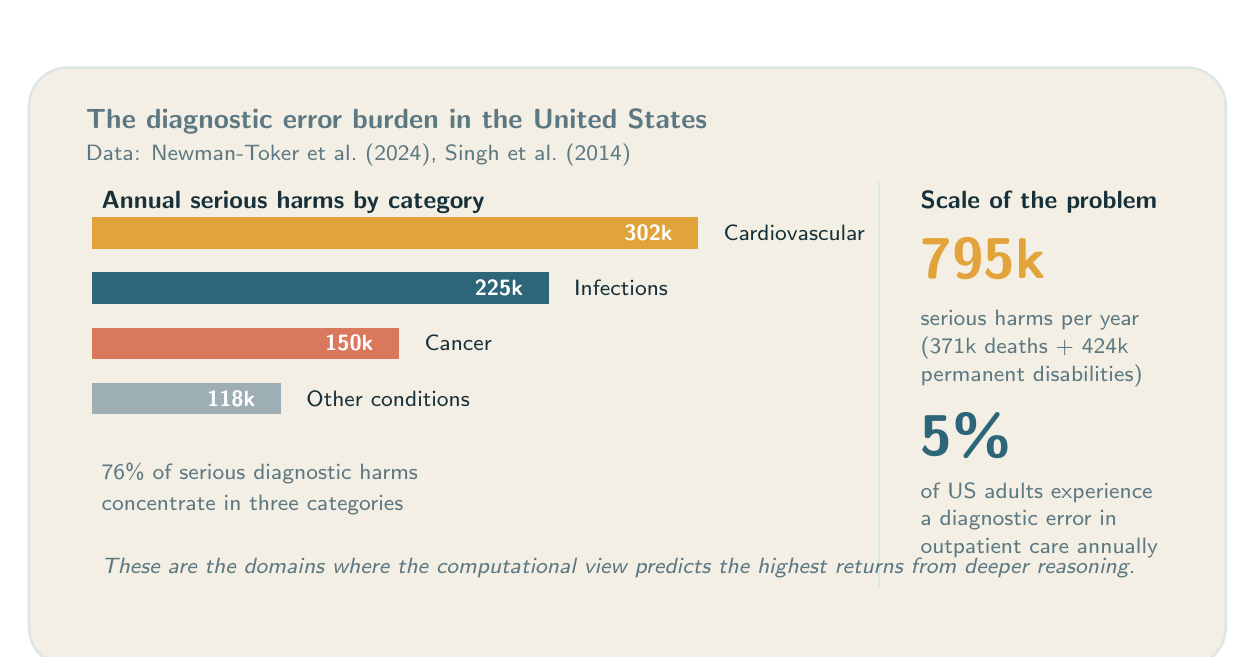
\begin{tikzpicture}[x=1cm,y=1cm]
  \fill[eirsand, rounded corners=14pt] (0,0) rectangle (15.2,7.6);
  \draw[eirmist, line width=0.9pt, rounded corners=14pt] (0,0) rectangle (15.2,7.6);

  % Title
  \node[anchor=north west, font=\bfseries\fontsize{10}{12}\selectfont, text=eirslate] at (0.6,7.2) {The diagnostic error burden in the United States};
  \node[anchor=north west, font=\fontsize{8}{10}\selectfont, text=eirslate] at (0.6,6.75) {Data: Newman-Toker et al.\ (2024), Singh et al.\ (2014)};

  % Left panel: bar chart of serious harms
  \node[anchor=north west, font=\bfseries\fontsize{9}{11}\selectfont, text=eirink] at (0.8,6.15) {Annual serious harms by category};

  % Bars (horizontal) — data from Newman-Toker: cardiovascular, infection, cancer = 76%
  \fill[eirgold] (0.8,5.3) rectangle (8.5,5.7);
  \node[anchor=west, font=\fontsize{8}{10}\selectfont, text=eirink] at (8.7,5.5) {Cardiovascular};
  \node[anchor=east, font=\bfseries\fontsize{8}{10}\selectfont, text=white] at (8.3,5.5) {302k};

  \fill[eirblue] (0.8,4.6) rectangle (6.6,5.0);
  \node[anchor=west, font=\fontsize{8}{10}\selectfont, text=eirink] at (6.8,4.8) {Infections};
  \node[anchor=east, font=\bfseries\fontsize{8}{10}\selectfont, text=white] at (6.4,4.8) {225k};

  \fill[eirrose] (0.8,3.9) rectangle (4.7,4.3);
  \node[anchor=west, font=\fontsize{8}{10}\selectfont, text=eirink] at (4.9,4.1) {Cancer};
  \node[anchor=east, font=\bfseries\fontsize{8}{10}\selectfont, text=white] at (4.5,4.1) {150k};

  \fill[eirslate!60] (0.8,3.2) rectangle (3.2,3.6);
  \node[anchor=west, font=\fontsize{8}{10}\selectfont, text=eirink] at (3.4,3.4) {Other conditions};
  \node[anchor=east, font=\bfseries\fontsize{8}{10}\selectfont, text=white] at (3.0,3.4) {118k};

  % Annotation
  \node[anchor=north west, font=\fontsize{8.5}{10.5}\selectfont, text=eirslate] at (0.8,2.7) {76\% of serious diagnostic harms};
  \node[anchor=north west, font=\fontsize{8.5}{10.5}\selectfont, text=eirslate] at (0.8,2.3) {concentrate in three categories};

  % Right panel: key numbers
  \draw[eirmist, line width=0.7pt] (10.8,1.0) -- (10.8,6.15);

  \node[anchor=north west, font=\bfseries\fontsize{9}{11}\selectfont, text=eirink] at (11.2,6.15) {Scale of the problem};

  \node[anchor=north west, font=\bfseries\fontsize{22}{26}\selectfont, text=eirgold] at (11.2,5.55) {795k};
  \node[anchor=north west, font=\fontsize{8.5}{10.5}\selectfont, text=eirslate] at (11.2,4.65) {serious harms per year};
  \node[anchor=north west, font=\fontsize{8.5}{10.5}\selectfont, text=eirslate] at (11.2,4.3) {(371k deaths + 424k};
  \node[anchor=north west, font=\fontsize{8.5}{10.5}\selectfont, text=eirslate] at (11.2,3.95) {permanent disabilities)};

  \node[anchor=north west, font=\bfseries\fontsize{22}{26}\selectfont, text=eirblue] at (11.2,3.35) {5\%};
  \node[anchor=north west, font=\fontsize{8.5}{10.5}\selectfont, text=eirslate] at (11.2,2.45) {of US adults experience};
  \node[anchor=north west, font=\fontsize{8.5}{10.5}\selectfont, text=eirslate] at (11.2,2.1) {a diagnostic error in};
  \node[anchor=north west, font=\fontsize{8.5}{10.5}\selectfont, text=eirslate] at (11.2,1.75) {outpatient care annually};

  % Bottom annotation
  \node[anchor=north west, font=\itshape\fontsize{8}{10}\selectfont, text=eirslate] at (0.8,1.5) {These are the domains where the computational view predicts the highest returns from deeper reasoning.};
\end{tikzpicture}
\caption{The diagnostic error burden concentrates in exactly the domains where the computational view predicts the highest compute elasticity. Data from Newman-Toker et al.\ \citep{newmantoker2024} and Singh et al.\ \citep{singh2014}.}
\label{fig:error_burden}
\end{figure}

\begin{figure}[t]
\centering
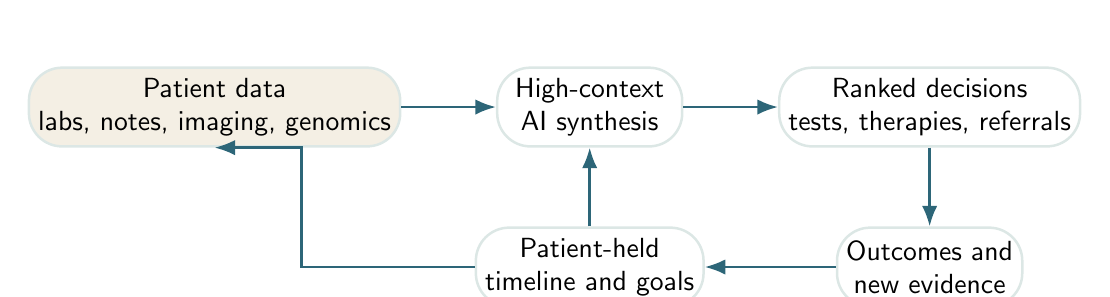
\begin{tikzpicture}[node distance=1.0cm]
  \tikzstyle{box}=[rounded corners=12pt, draw=eirmist, line width=0.9pt, fill=white, minimum width=2.35cm, minimum height=1cm, align=center]
  \tikzstyle{arrow}=[-{Latex[length=2.6mm]}, line width=0.9pt, color=eirblue]

  \node[box, fill=eirsand] (data) {Patient data\\labs, notes, imaging, genomics};
  \node[box, right=1.2cm of data] (synthesis) {High-context\\AI synthesis};
  \node[box, right=1.2cm of synthesis] (decision) {Ranked decisions\\tests, therapies, referrals};
  \node[box, below=1.0cm of decision] (feedback) {Outcomes and\\new evidence};
  \node[box, below=1.0cm of synthesis] (patient) {Patient-held\\timeline and goals};

  \draw[arrow] (data) -- (synthesis);
  \draw[arrow] (synthesis) -- (decision);
  \draw[arrow] (decision) -- (feedback);
  \draw[arrow] (feedback) -- (patient);
  \draw[arrow] (patient) -- (synthesis);
  \draw[arrow] (patient.west) -| ++(-2.2,0) |- (data.south);
\end{tikzpicture}
\caption{The patient-compute loop. In high-burden disease, value comes from repeated synthesis over the full timeline rather than one-shot question answering.}
\label{fig:loop}
\end{figure}

\section{Why patient-held data matter}
Clinical reasoning is not a single-agent process. It is distributed across general practitioners, specialists, pathologists, radiologists, and multidisciplinary teams. Each referral is a computational step; each handoff is a potential information loss. The rare-disease ``diagnostic odyssey''---averaging 7 years and 15 referrals---is not a story about one doctor who failed to think hard enough. It is a distributed search that could not maintain state across its own nodes: hypotheses dropped at specialty boundaries, prior exclusions repeated because no entity held the full search history.

AI is uniquely positioned to hold the full search state together across fragmented care. The patient is the only entity that persists across all episodes, making them the natural locus of computational state. Once patients can assemble data across encounters, institutions, and modalities, compute moves with the patient rather than remaining trapped inside an institution. OpenNotes showed that patients value direct access to clinicians' notes and that transparency improves engagement \citep{delbanco2010}. Patients shared those notes with family and caregivers, turning records into coordination artifacts \citep{jackson2014}. Patient-generated data---symptom tracking, wearables, home monitoring---are increasingly common \citep{park2018}. Records are no longer only institutional memory; they are becoming a substrate for continuous reasoning.

Raw access is not enough. Precision medicine remains incomplete without patients as active participants in data interpretation \citep{tuttle2021}. AI for shared decision-making must improve deliberation, not simply generate recommendations \citep{hassan2024}. Integration of patient-generated health data is not merely a technical challenge but a clinical, organizational, and evidentiary one \citep{jim2020}. Early work shows patients can already use large language models on open notes to interpret their records \citep{salmi2025}---early evidence, not clinical validation, but it clarifies the direction. Once patients can access their full timeline, the missing layer is repeatable reasoning over it.

\subsection{Counterarguments and constraints}
Patient-held data are not automatically useful. Provenance may be uncertain, timestamps incomplete, self-tracked measures drifting, and the patients most likely to benefit may face the largest barriers in digital access \citep{huckvale2019}. The computational paradigm depends on a stricter standard than interoperability: provenance, chronology, validation, and interfaces that separate observed evidence from inferred conclusions.

\summarybox{
\textbf{Access versus leverage.} Data access creates possibility. Computational interpretation creates leverage. In a patient-centered health stack, the two should be designed together.
}

\section{Evidence from the highest-leverage domains}

\subsection{Precision oncology}
Cancer is already a computational problem. Molecular diagnosis, resistance interpretation, treatment sequencing, and trial matching require synthesis across pathology, imaging, genomics, prior therapy, and time. Personalized cancer vaccines make this explicit: identifying patient-specific tumor mutations, ranking neoantigens, and manufacturing a bespoke intervention. Sahin and colleagues showed that individualized RNA mutanome vaccines mobilize poly-specific immunity against melanoma \citep{sahin2017}. AlphaFold expands the search surface further by making protein consequence analysis tractable across large molecular spaces \citep{jumper2021}.

Compute sits inside the decision itself: which mutation matters, which escape mechanisms are plausible, which combination is worth pursuing, which trial is defensible for this patient now. The burden of reasoning has become part of the disease burden.

A single patient may generate surgical pathology, radiology progression patterns, panel sequencing, circulating tumor DNA, treatment toxicities, and eligibility-relevant comorbidities. The computational task is to rank drivers, resistance hypotheses, and therapeutic branches while making uncertainty visible. The leverage comes not from generating prose about cancer but from compressing a large search problem into a smaller set of defensible next moves.

\subsection{Rare disease genomics}
The problem is not only finding a variant but aligning phenotype, pedigree, prior negative workup, and the literature fast enough to affect care. Wojcik and colleagues showed in the \emph{New England Journal of Medicine} that genome sequencing materially improved diagnosis for suspected rare disease \citep{wojcik2024}. This is a canonical compute-heavy domain: large hypothesis spaces, sparse signal, fragmented records, and a direct payoff when reasoning succeeds. The cost of failure is now quantified: rare-disease patients accumulate average healthcare costs of \euro{27,000} over their diagnostic odyssey, compared to \euro{3,600} for matched controls, and avoidable costs of delayed diagnosis in the US range from \$86,000 to over \$517,000 per patient \citep{glaubitz2025}.

\subsection{Resistant infection and antibiotic discovery}
Antimicrobial resistance presents a two-layer search problem. The first is patient-specific: organism identity, susceptibility, host state, prior exposure, organ function, and drug interactions. The second is discovery: searching chemical space for compounds with novel activity. Stokes and colleagues used deep learning to identify halicin, accelerating antibiotic discovery in regions of chemical space invisible to standard pipelines \citep{stokes2020}. More compute means better regimen ranking in the clinic and better exploration of candidate space in the lab.

\subsection{Sepsis and critical care}
In critical care the challenge is time. Dozens of measurements update continuously, and the relevant signal is distributed across trends rather than single observations. A machine-learning sepsis early-warning system deployed across multiple hospitals was associated with faster antibiotic administration and lower mortality \citep{adams2022}. Deep learning on electronic health records can scale across broad clinical prediction tasks using the raw longitudinal record \citep{rajkomar2018}, and pragmatic deterioration surveillance can attach to live escalation pathways \citep{moses2025}. These results establish that longitudinal records contain actionable signal, and systems that hold more context together improve timing-sensitive decisions.

\subsection{Psychiatry and mental health}
Psychiatry may be the most computationally complex domain in medicine. First-line antidepressants fail in roughly half of patients; the standard of care is brute-force search through medication options over months, each failed trial costing time, side effects, and continued illness. Pharmacogenomics offers a partial shortcut: variation in cytochrome P450 enzymes can predict whether a patient will metabolize a medication too quickly, too slowly, or normally, eliminating likely failures before they are tried \citep{hicks2015}. The bottleneck is not genotyping---that is cheap---but integration: connecting genotype to drug list to patient history to prescribing decision.

The deeper computational burden extends beyond drug selection. The relevant search space in psychiatry is not a genome or a set of lab values. It is the patient's entire cognitive and experiential landscape: learned patterns, coping strategies, relational templates, and interpretive habits shaped by a lifetime. Many mental health conditions are maladaptive but semi-stable states---locally reinforced ways of interacting with the world that persist because they reduce short-term distress while deepening long-term dysfunction. Social anxiety drives avoidance, which prevents disconfirmation. Depression drives withdrawal, which eliminates sources of reinforcement. These are local minima in a behavioral landscape: stable enough to resist casual intervention, but not globally optimal.

Cognitive behavioral therapy makes this computational structure explicit. The ABC model---antecedent, behavior, consequence---is a structured search through cognitive patterns: identify triggers, map responses, trace reinforcing consequences, and find the self-sustaining loops that maintain the disorder \citep{beck2005}. The therapist's task is a search over a high-dimensional space defined by the patient's beliefs, behaviors, and context, seeking patterns that, if restructured, would shift the patient from a maladaptive equilibrium to a more adaptive one. More careful exploration of this landscape changes the outcome.

The latent demand for computational support is already visible: a large fraction of general-purpose LLM users turn to them for emotional support and self-reflection. This is not validated therapy, but it reveals that people intuit cognitive pattern work as a reasoning process and reach for computational tools when human reasoning time is unavailable.

Psychiatry is not a marginal case for the computational view. It is one of its most demanding tests: iterative search over the full landscape of human cognition, behavior, and experience.

\subsection{Patient-reported outcomes and symptom monitoring}
Not all high-value computation depends on genomics. Electronic patient-reported symptom monitoring during cancer treatment improved overall survival, likely by enabling earlier response to deterioration patterns otherwise missed \citep{basch2016,basch2017}. Symptoms, side effects, and tolerability live outside the hospital until severe enough to trigger contact. In the computational paradigm, those signals become first-class inputs into the case model.

\section{N-of-1 medicine and personal computation}
The computational view converges with N-of-1 medicine. Schork argued that precision medicine must be understood at the level of the individual, not the cohort average \citep{schork2015}. Guyatt laid the foundation for randomized trials in individual patients \citep{guyatt1986}; Lillie argued that N-of-1 trials align with the actual endpoint of clinical practice: optimizing care for one person \citep{lillie2011}. Augustine proposed a roadmap for N-of-1 therapies covering scientific, operational, and regulatory requirements \citep{augustine2024}; Jonker outlined how N-of-1 medicine could reshape treatment evaluation for rare and heterogeneous disease \citep{jonker2025}. These contributions move personalization from slogan to organizing scientific unit.

Longitudinal self-measurement provides parallel evidence. Integrative personal omics profiling reveals dynamic molecular phenotypes within a single individual over time \citep{chen2012}. Dense personal data clouds can monitor health transitions with temporal resolution far exceeding episodic care \citep{piening2018}. Biology, symptoms, and risk are often more legible in longitudinal within-person data than in sparse snapshots.

Public self-experimentation---highly instrumented programmes such as Bryan Johnson's---is not clinical evidence. What it reveals is latent demand: people want to run dense longitudinal data loops over their own bodies. The scientific path forward is audited N-of-1 workflows combining patient goals, validated measurements, and clinically accountable reasoning.

\section{Case examples}
Table~\ref{tab:cases} shows why a single computational model fits these otherwise different domains.\vspace{-0.3em}

\begin{table}[t]
\centering
\small
\begin{tabularx}{\textwidth}{>{\raggedright\arraybackslash}p{2.5cm} >{\raggedright\arraybackslash}p{2.7cm} >{\raggedright\arraybackslash}X >{\raggedright\arraybackslash}p{2.5cm}}
\toprule
\textbf{Domain} & \textbf{Core data} & \textbf{How computation is leveraged} & \textbf{Representative evidence} \\
\midrule
Precision oncology & Genomics, pathology, imaging, treatment history & Variant interpretation, resistance modeling, neoantigen ranking, regimen sequencing, trial matching & \citet{sahin2017}; \citet{jumper2021} \\
Rare disease & Phenotype timeline, pedigree, genome sequencing, prior workup & Cross-linking phenotype ontologies, literature, family history, and candidate variants & \citet{wojcik2024} \\
Resistant infection & Microbiology, susceptibilities, organ function, prior antibiotic exposure & Better ranking of therapies and faster search across compound or regimen space & \citet{stokes2020} \\
Sepsis / ICU & Streaming vitals, labs, notes, medication events & Earlier escalation from weak, time-distributed patterns across the longitudinal record & \citet{adams2022}; \citet{rajkomar2018}; \citet{moses2025} \\
Patient-reported symptoms & Patient-reported outcomes, treatments, toxicities, goals & Detecting deterioration and treatment intolerance before they become acute & \citet{basch2016}; \citet{basch2017} \\
Patient-held records & Notes, meds, labs, imaging reports, symptoms, goals & Converts raw data access into usable reasoning leverage before and between encounters & \citet{delbanco2010}; \citet{salmi2025} \\
\bottomrule
\end{tabularx}
\caption{High-value disease areas under a computational lens.}
\label{tab:cases}
\end{table}

\begin{figure}[t]
\centering
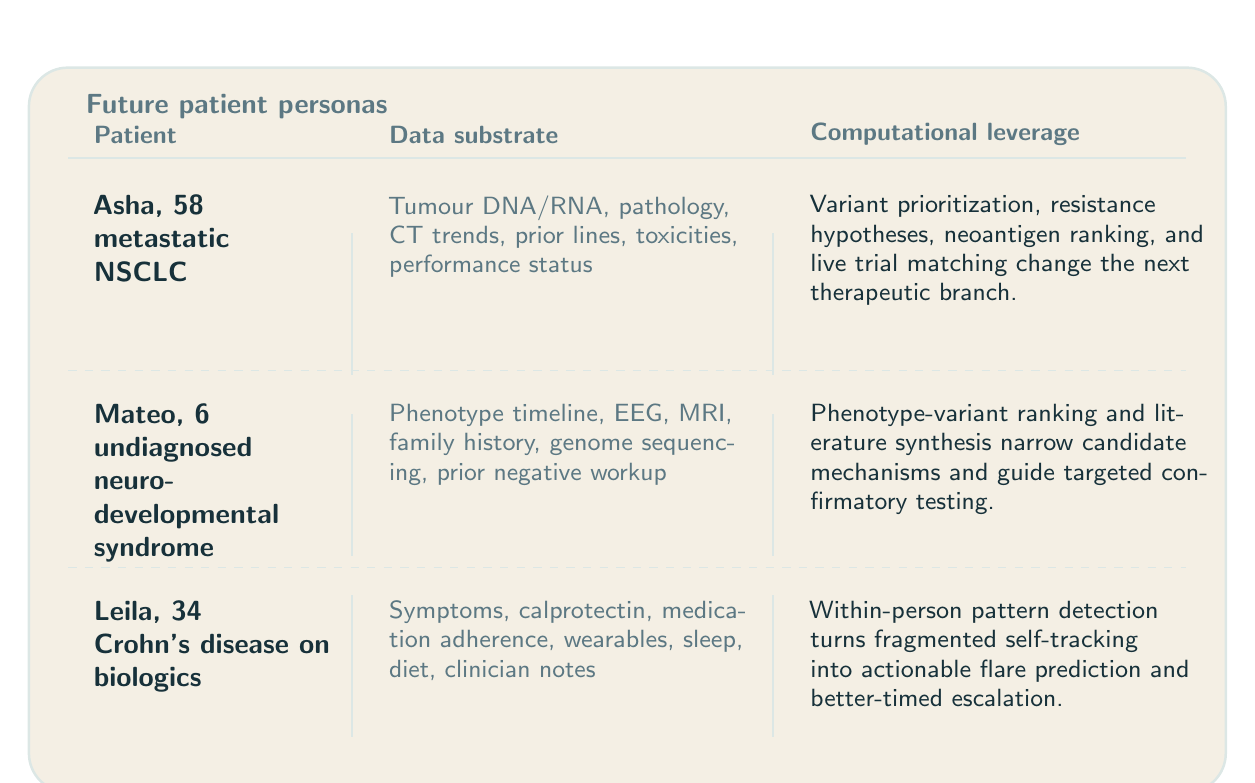
\begin{tikzpicture}[x=1cm,y=1cm]
  \fill[eirsand, rounded corners=14pt] (0,0) rectangle (15.2,9.2);
  \draw[eirmist, line width=0.9pt, rounded corners=14pt] (0,0) rectangle (15.2,9.2);

  \foreach \y in {6.2,3.9,1.6} {
    \draw[eirmist, line width=0.7pt] (4.1,\y+0.9) -- (4.1,\y-0.9);
    \draw[eirmist, line width=0.7pt] (9.45,\y+0.9) -- (9.45,\y-0.9);
  }

  \node[anchor=west, font=\bfseries\fontsize{10}{12}\selectfont, text=eirslate] at (0.6,8.7) {Future patient personas};
  \draw[eirmist, line width=0.7pt] (0.5,8.05) -- (14.7,8.05);
  \node[anchor=west, font=\bfseries\fontsize{9}{11}\selectfont, text=eirslate] at (0.7,8.35) {Patient};
  \node[anchor=west, font=\bfseries\fontsize{9}{11}\selectfont, text=eirslate] at (4.45,8.35) {Data substrate};
  \node[anchor=west, font=\bfseries\fontsize{9}{11}\selectfont, text=eirslate] at (9.8,8.35) {Computational leverage};

  \node[anchor=north west, text width=3.0cm, align=left, font=\bfseries\fontsize{10}{12}\selectfont, text=eirink] at (0.7,7.7) {Asha, 58\\metastatic NSCLC};
  \node[anchor=north west, text width=4.55cm, align=left, font=\fontsize{8.7}{10.6}\selectfont, text=eirslate] at (4.45,7.7) {Tumour DNA/RNA, pathology, CT trends, prior lines, toxicities, performance status};
  \node[anchor=north west, text width=5.0cm, align=left, font=\fontsize{8.7}{10.6}\selectfont, text=eirink] at (9.8,7.7) {Variant prioritization, resistance hypotheses, neoantigen ranking, and live trial matching change the next therapeutic branch.};

  \draw[eirmist, line width=0.5pt, dashed] (0.5,5.35) -- (14.7,5.35);

  \node[anchor=north west, text width=3.0cm, align=left, font=\bfseries\fontsize{10}{12}\selectfont, text=eirink] at (0.7,5.05) {Mateo, 6\\undiagnosed neuro-\newline developmental syndrome};
  \node[anchor=north west, text width=4.55cm, align=left, font=\fontsize{8.7}{10.6}\selectfont, text=eirslate] at (4.45,5.05) {Phenotype timeline, EEG, MRI, family history, genome sequencing, prior negative workup};
  \node[anchor=north west, text width=5.0cm, align=left, font=\fontsize{8.7}{10.6}\selectfont, text=eirink] at (9.8,5.05) {Phenotype-variant ranking and literature synthesis narrow candidate mechanisms and guide targeted confirmatory testing.};

  \draw[eirmist, line width=0.5pt, dashed] (0.5,2.85) -- (14.7,2.85);

  \node[anchor=north west, text width=3.0cm, align=left, font=\bfseries\fontsize{10}{12}\selectfont, text=eirink] at (0.7,2.55) {Leila, 34\\Crohn's disease on biologics};
  \node[anchor=north west, text width=4.55cm, align=left, font=\fontsize{8.7}{10.6}\selectfont, text=eirslate] at (4.45,2.55) {Symptoms, calprotectin, medication adherence, wearables, sleep, diet, clinician notes};
  \node[anchor=north west, text width=5.0cm, align=left, font=\fontsize{8.7}{10.6}\selectfont, text=eirink] at (9.8,2.55) {Within-person pattern detection turns fragmented self-tracking into actionable flare prediction and better-timed escalation.};
\end{tikzpicture}
\caption{Concrete personas for a computational health stack. The same design principle appears across specialties: assemble the full timeline, compute over it repeatedly, and use the result to improve the next decision.}
\label{fig:personas}
\end{figure}

\subsection{Concrete pathways}
In each case, computation improves preparation, ranking, and timing for the next branch in care---not to replace the clinician but to strengthen the decision.

\begin{enumerate}
  \item \textbf{Precision oncology.} A patient-assembled case file combines sequencing, pathology, imaging, and prior therapies. Compute ranks drivers, resistance mechanisms, toxic trade-offs, and live trials. The output is a defensible next branch with explicit uncertainty.
  \item \textbf{Rare disease.} A phenotype timeline with milestones, regressions, imaging, and prior exclusions is linked to genome evidence and literature, eliminating time spent re-deriving the case at each referral.
  \item \textbf{Chronic inflammatory disease.} Symptoms, labs, wearable data, and medication exposure are integrated within-person to identify precursors of flare, intolerance, or non-response.
\end{enumerate}

\begin{table}[t]
\centering
\small
\begin{tabularx}{\textwidth}{>{\raggedright\arraybackslash}p{3.2cm} >{\raggedright\arraybackslash}p{4.2cm} >{\raggedright\arraybackslash}X}
\toprule
\textbf{Study type} & \textbf{What changed} & \textbf{Why it matters for the thesis} \\
\midrule
Pragmatic randomized clinical trial in cardiovascular screening & AI-enabled ECG alerts were tested as an intervention rather than a retrospective classifier \citep{lin2024} & Supports the claim that computational systems can change downstream decisions and outcomes, not merely generate scores. \\
Pragmatic cluster-randomized deterioration trial & Real-time surveillance for patient deterioration was tested across live inpatient settings \citep{moses2025} & Strengthens the case that high-context clinical surveillance can function as an operational care system. \\
Patient-record sharing study & Patients with transparent notes shared them with family and caregivers, extending the practical reach of the record \citep{jackson2014} & Shows that once patients have access to records, those records begin acting as coordination infrastructure. \\
Patient-side LLM proof of concept & Patients used large language models on open notes to better understand and work with their records \citep{salmi2025} & Gives direct support to the argument that personal compute can become part of the patient toolkit. \\
\bottomrule
\end{tabularx}
\caption{Evidence that the computational view extends beyond retrospective prediction.}
\label{tab:intervention}
\end{table}

\begin{figure}[t]
\centering
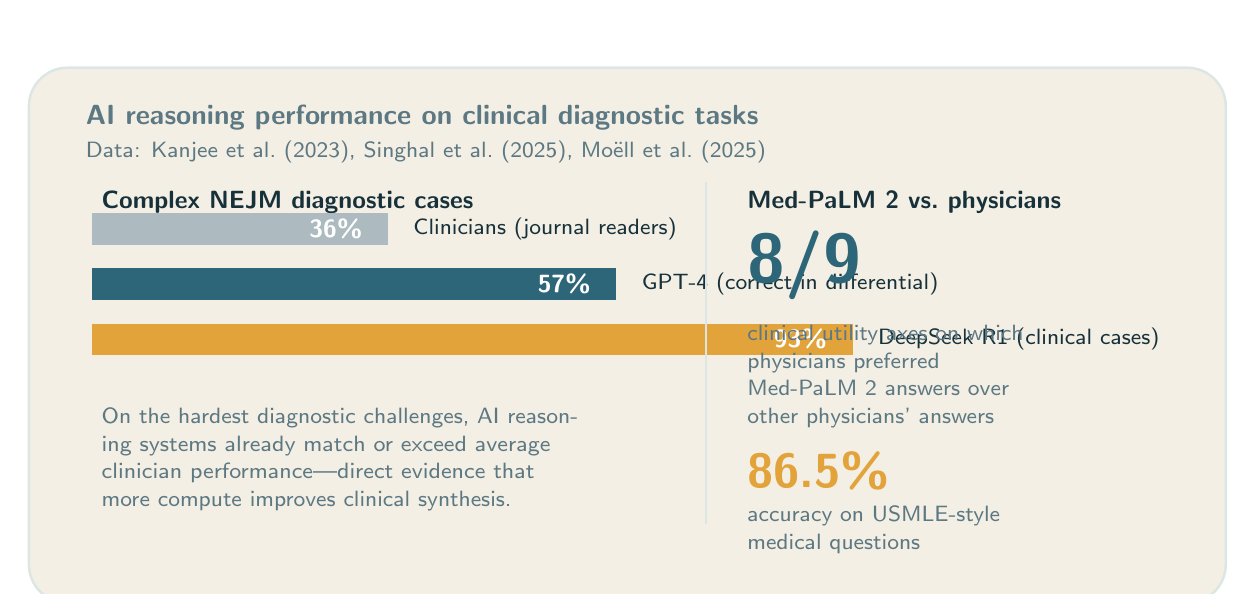
\begin{tikzpicture}[x=1cm,y=1cm]
  \fill[eirsand, rounded corners=14pt] (0,0) rectangle (15.2,6.8);
  \draw[eirmist, line width=0.9pt, rounded corners=14pt] (0,0) rectangle (15.2,6.8);

  % Title
  \node[anchor=north west, font=\bfseries\fontsize{10}{12}\selectfont, text=eirslate] at (0.6,6.45) {AI reasoning performance on clinical diagnostic tasks};
  \node[anchor=north west, font=\fontsize{8}{10}\selectfont, text=eirslate] at (0.6,6.0) {Data: Kanjee et al.\ (2023), Singhal et al.\ (2025), Mo\"ell et al.\ (2025)};

  % Left panel: NEJM case challenges (Kanjee)
  \node[anchor=north west, font=\bfseries\fontsize{9}{11}\selectfont, text=eirink] at (0.8,5.35) {Complex NEJM diagnostic cases};

  % Clinician bar
  \fill[eirslate!50] (0.8,4.55) rectangle (4.56,4.95);
  \node[anchor=east, font=\bfseries\fontsize{9}{11}\selectfont, text=white] at (4.36,4.75) {36\%};
  \node[anchor=west, font=\fontsize{8}{10}\selectfont, text=eirink] at (4.76,4.75) {Clinicians (journal readers)};

  % GPT-4 bar
  \fill[eirblue] (0.8,3.85) rectangle (7.46,4.25);
  \node[anchor=east, font=\bfseries\fontsize{9}{11}\selectfont, text=white] at (7.26,4.05) {57\%};
  \node[anchor=west, font=\fontsize{8}{10}\selectfont, text=eirink] at (7.66,4.05) {GPT-4 (correct in differential)};

  % DeepSeek R1 bar
  \fill[eirgold] (0.8,3.15) rectangle (10.46,3.55);
  \node[anchor=east, font=\bfseries\fontsize{9}{11}\selectfont, text=white] at (10.26,3.35) {93\%};
  \node[anchor=west, font=\fontsize{8}{10}\selectfont, text=eirink] at (10.66,3.35) {DeepSeek R1 (clinical cases)};

  % Annotation
  \node[anchor=north west, text width=6cm, font=\fontsize{8}{10}\selectfont, text=eirslate] at (0.8,2.6) {On the hardest diagnostic challenges, AI reasoning systems already match or exceed average clinician performance---direct evidence that more compute improves clinical synthesis.};

  % Right panel: Med-PaLM 2
  \draw[eirmist, line width=0.7pt] (8.6,1.0) -- (8.6,5.35);

  \node[anchor=north west, font=\bfseries\fontsize{9}{11}\selectfont, text=eirink] at (9.0,5.35) {Med-PaLM 2 vs.\ physicians};

  \node[anchor=north west, font=\bfseries\fontsize{28}{32}\selectfont, text=eirblue] at (9.0,4.85) {8/9};
  \node[anchor=north west, text width=5cm, font=\fontsize{8.5}{10.5}\selectfont, text=eirslate] at (9.0,3.65) {clinical utility axes on which};
  \node[anchor=north west, text width=5cm, font=\fontsize{8.5}{10.5}\selectfont, text=eirslate] at (9.0,3.3) {physicians preferred};
  \node[anchor=north west, text width=5cm, font=\fontsize{8.5}{10.5}\selectfont, text=eirslate] at (9.0,2.95) {Med-PaLM 2 answers over};
  \node[anchor=north west, text width=5cm, font=\fontsize{8.5}{10.5}\selectfont, text=eirslate] at (9.0,2.6) {other physicians' answers};

  \node[anchor=north west, font=\bfseries\fontsize{18}{22}\selectfont, text=eirgold] at (9.0,2.05) {86.5\%};
  \node[anchor=north west, text width=5cm, font=\fontsize{8.5}{10.5}\selectfont, text=eirslate] at (9.0,1.35) {accuracy on USMLE-style};
  \node[anchor=north west, text width=5cm, font=\fontsize{8.5}{10.5}\selectfont, text=eirslate] at (9.0,1.0) {medical questions};
\end{tikzpicture}
\caption{AI reasoning systems match or exceed clinician performance on complex diagnostic benchmarks. Data from Kanjee et al.\ \citep{kanjee2023}, Singhal et al.\ \citep{singhal2025}, and Mo\"ell et al.\ \citep{moell2025reasoning}. These results support the thesis that additional inference---more compute applied to clinical reasoning---improves decision quality.}
\label{fig:ai_performance}
\end{figure}

\section{Evaluation and endpoints}
The computational view should change how health AI is evaluated. Discrimination metrics are not enough. In high-stakes medicine, calibration matters as much as accuracy: a system that outputs ``60\% diagnosis A, 25\% diagnosis B, and here is the test that discriminates'' is more useful than a bare point estimate, even at identical accuracy. More reasoning sometimes does not change the top-ranked answer but sharpens the uncertainty estimate, which clinically determines whether a clinician orders a confirmatory test, refers, or treats empirically. The relevant question is whether synthesis quality---including calibration---improved at the point where the case could still change direction.

\begin{table}[t]
\centering
\small
\begin{tabularx}{\textwidth}{>{\raggedright\arraybackslash}p{3.0cm} >{\raggedright\arraybackslash}p{4.1cm} >{\raggedright\arraybackslash}X}
\toprule
\textbf{Domain} & \textbf{Primary endpoint candidates} & \textbf{Why these endpoints fit the computational thesis} \\
\midrule
Rare disease & Time to diagnosis; diagnostic yield; avoided procedures & Measures whether synthesis reduced time spent on the wrong branch of care. \\
Precision oncology & Time to molecular recommendation; trial-match yield; change in treatment ranking; time to next line & Measures whether computation improved branching decisions rather than documentation alone. \\
Sepsis / ICU & Time to escalation; antibiotics or intervention timing; false alerts per patient-day; mortality or ICU transfer & Measures whether longitudinal synthesis improved timing without overwhelming workflow. \\
Chronic disease / N-of-1 care & Time to flare detection; within-person treatment response; symptom burden; adherence to preferred regimen & Measures whether repeated computation improves individualized management over time. \\
Patient-facing record synthesis & Patient comprehension; visit preparedness; question quality; fewer duplicated tests; continuity across sites & Measures whether access plus reasoning improved the practical utility of records. \\
\bottomrule
\end{tabularx}
\caption{Evaluation endpoints aligned with a computational view of medicine. The goal is to measure whether reasoning improves decisions, not only whether predictions look accurate offline.}
\label{tab:endpoints}
\end{table}

\calloutbox{Illustrative translational case}{
A widely discussed 2025 media report described how an Australian entrepreneur used sequencing, variant analysis, and AI-assisted reasoning to help design a personalized mRNA treatment strategy for his dog Rosie, who had a mast cell tumour \citep{abc2025rosie}. This is not high-level evidence in the way a randomized trial is. It is useful for a different reason: it makes visible what the computational workflow looks like once motivated people can assemble data, models, and synthesis outside a traditional institutional pipeline.
}

\section{What should be built}
Health systems, startups, and regulators should prioritize tools that make high-burden reasoning portable, inspectable, and patient-aligned---not chatbots, but reasoning infrastructure.

\begin{enumerate}
  \item \textbf{Patient-assembled case files.} Systems should ingest records from multiple providers and preserve chronology rather than flattening everything into isolated visits.
  \item \textbf{Explicit uncertainty handling.} Models should separate evidence, inference, and missing information, especially in oncology, genetics, psychiatry, and infection.
  \item \textbf{Decision-oriented outputs.} The output should not just summarize. It should rank the next tests, consultations, or therapeutic branches.
  \item \textbf{Re-runnable reasoning.} Every major disease course changes over time. The right unit is a living case model, not a one-time answer.
  \item \textbf{Patient-clinician collaboration.} The design target is a stronger clinical conversation, not consumer isolation.
  \item \textbf{N-of-1 evidence layers.} Systems should support repeated within-person hypothesis testing when disease is relapsing, heterogeneous, or highly treatment-sensitive.
\end{enumerate}

\section{Risks and constraints}
The computational view sharpens the need for evidence and oversight. High-burden disease is where hallucinated synthesis, hidden bias, dataset shift, and brittle prompting are most dangerous. Reasoning systems must be auditable, source-grounded, and explicit about what they do not know.

If compute improves outcomes, unequal access to compute becomes a health inequity. A health stack that gives patients records but not synthesis leaves too much leverage with the institution.

Some biological processes may be computationally irreducible: no model can predict their trajectory faster than the process itself. Immune response to a novel pathogen, idiosyncratic drug reactions, the nonlinear dynamics of some cancers---these may resist predictive compression regardless of inference applied. Compute elasticity is not universally high. The computational view is a claim about where the bottleneck lies \emph{when it lies in reasoning}, not a claim that reasoning is always the bottleneck.

``Personalization'' in this paradigm is not a user-experience feature. It is a property of the reasoning problem: requiring timeline integrity, provenance, repeated re-analysis, and outcome feedback.

\section{Operational consequences}
The agenda for health AI changes. Product teams should stop treating every workflow as though it deserves the same model complexity. Clinical systems should separate protocol problems from search problems. Regulators should ask whether a model improves reasoning quality in the cases where reasoning is the bottleneck, not only whether it is accurate on average.

The economics are stark. A rare-disease diagnostic odyssey averages seven years and tens of thousands of dollars in unnecessary procedures. An AI system that compresses that timeline might cost tens of dollars in compute. A missed oncology trial match means a patient who might have responded never receives the therapy; the value of a correct match dwarfs the cost of computation. Each failed antidepressant trial costs six to eight weeks of illness; pharmacogenomic testing costs two hundred dollars. The ratio between the cost of reasoning and the cost of its absence is routinely one hundred to one or higher.

Medicine is organized around the assumption that reasoning is expensive and scarce. This scarcity shapes the referral hierarchy, the fifteen-minute consultation, the division between generalists and specialists, and the requirement that patients travel to access expert judgment. Cheap, portable AI reasoning changes these structures. Referrals become less necessary when generalists access specialist-level synthesis. Consultations shift from racing to integrate data toward judgment over pre-computed analysis. The medical record transforms from stored document to computational substrate. Geography becomes less binding: a rural clinic accesses the same synthesis depth as an academic center. The binding constraint shifts from proximity to experts to data quality and action capacity. This is the deeper paradigm shift: cheap computation restructures how medical reasoning is distributed across people, machines, time, and institutions.

The practical payoff is concentration. Compute should go where it buys something real: fewer missed mutations, faster rare-disease diagnoses, better antibiotic choices, earlier sepsis escalation, systematic medication sequencing in psychiatry, and better continuity across fragmented care. Pragmatic intervention studies in ECG alerting, deterioration surveillance, and symptom monitoring show this shift can move from theory to operations when attached to real decision paths \citep{lin2024,moses2025,basch2016}.

\calloutbox{Testable predictions}{
\textbf{Prediction 1.} Within five years, the most effective clinical AI deployments will increasingly be evaluated on time-to-decision and branch-quality endpoints rather than stand-alone discrimination metrics.\\
\textbf{Prediction 2.} The first widely adopted patient-facing AI tools in medicine will succeed not as synthetic clinicians but as timeline integrators and case-preparation systems.\\
\textbf{Prediction 3.} N-of-1 computational care loops will emerge first in rare disease, oncology, and relapsing chronic disease, where within-person variation and high decision burden are most visible.\\
\textbf{Prediction 4.} Institutions that expose records without exposing usable reasoning will create a new form of incomplete patient empowerment.
}

\section{Conclusion}
Medicine is already a computational process. It has been one since the first clinician held two observations in mind and asked which diagnosis fit better. Evidence-based medicine formalized this at the population level. The computational view proposed here formalizes it at the patient level, and argues that the gap between what is currently computed and what could be computed is the single largest source of avoidable harm in complex disease.

The diseases that matter most under this view are not simply the most prevalent. They are the ones that become search problems when viewed at patient resolution---where the hypothesis space is large, the evidence is distributed, and the quality of reasoning directly determines whether the patient ends up on the right branch of care or the wrong one. Precision oncology, rare-disease genomics, resistant infection, psychiatric treatment selection, selected critical care settings, and chronic relapsing diseases are early proof that this lens is practical rather than rhetorical.

The deeper implication is structural. If reasoning has historically been scarce and expensive---bound to the time, memory, and attention of individual clinicians---then cheap, portable computation changes not only the quality of individual decisions but the architecture of medicine itself: how referrals work, what consultations are for, who can access specialist-level synthesis, and whether the medical record is a static archive or a living computational substrate.

That is why a computational view of medicine matters. It provides a principled way to measure where additional inference can genuinely change outcomes, a framework for directing resources toward the cases where the reasoning deficit is largest, and a vision for how health understanding can become a shared, longitudinal, patient-held capability rather than a privilege of the institution. The question is no longer whether medicine will become more computational. It is how fast, how equitably, and how well.

\bibliographystyle{plainnat}
\bibliography{references}

\end{document}
